\documentclass{report}

\pagenumbering{gobble}
\usepackage[english]{babel}
\usepackage[pdftex]{color,graphicx}
\usepackage{enumitem}
\usepackage{pdfpages}
\setitemize{noitemsep,topsep=0pt,parsep=0pt,partopsep=0pt}
\setenumerate{noitemsep,topsep=0pt,parsep=0pt,partopsep=0pt}
\setlist[itemize]{leftmargin=*,noitemsep}
\usepackage[T1]{fontenc}

\title{Scientific Software Installation in the User Space\\
       \large A tutorial proposal for PEARC'21
			 }

\author{Ketan Maheshwari and Hong Liu\\ Oak Ridge National Laboratory}

\begin{document}
\maketitle
\section*{Abstract}
We propose to offer a comprehensive, definitive and clarifying tutorial on the
process and practice of scientific software building, installation,
configuration and setup in the \emph{user-space} for large-scale computational
infrastructures. The tutorial is motivated by authors' combined 10+ years of
experience working with science users addressing software related challenges.

\section*{Detailed description}
Scientific software installation process is often taken for granted.
Consequently, installations end up being suboptimal resulting in an underperforming
or worse, erratic software. Furthermore, a subpar installation often undergoes through faulty
post-install configuration, patches, etc. causing further degradation.

As the technical installation methods vary from software to software, the
process gets difficult and tedious that discourages users from installing some
packages on their own. This results in users stuck with older versions of
software preventing them from exploring newer features. In many cases, users
rely on sysadmins for such installs but this either causes delays or limited
installs owing to limited sysadmin hours at a typical computing center. 

With the advent of the python ecosystem, and a number of supported install methods
the waters have muddied quite a bit that often makes users resisting installing
software or face difficulties after a faulty installation due to conflicting
methods. It might even be impractical to install some such packages at system
level forcing users to install them in user-space. Many problems in python
ecosystems could be traced to a faulty installation which when properly
addressed solves them.

Our tutorial is a result of 10+ years of combined experience installing and
setting up a wide variety of software packages for self and domain users over a
number of cluster and supercomputing environments. We bring clarity to the
various software installation paradigms and give structure to a process that is
often perceived chaotic and irregular (which we believe is true to some
extent).

\subsection*{Tutorial goals}
\begin{enumerate}
\item To comprehensively cover, document and present the facets of the process and practice of scientific software installation.
\item Share knowledge of scientific software installation in user space over compute clusters and supercomputers.
\item Demonstrate best practices for software installation.
\item Clarify the concepts, principles and patterns found in the software installation process.
\item Present plenty of practical and hands-on examples of contemporary scientific software installation process.
\end{enumerate}

\subsection*{Relevance of topic to conference attendees}
We believe the topic is relevant and useful to conference attendees. The following scenarios support our belief:
\begin{itemize}
\item A researcher experimenting with several versions of a software library would like to efficiently install them in their home area.
\item A scientist who extends a popular scientific software and would like to link it to a cluster installed library.
\item Users who would like to use specialized compilers such as NAG or PGI that are not always available systemwide.
\item Users who would like to supplement the system installed libraries for GPUs with their own Kokkos driven codes.
\item Clarification on what is happening under the hood when issuing command
such as \texttt{pip3 install torch==1.0.1 -f
https://download.pytorch.org/whl/cu92/stable --user} which in turn will help
users understand the finer details of their python environment. 
\end{itemize}

\subsection*{Targeted audience}
\begin{itemize}
\item Users of Research Computing Centers will benefit with a clear understanding of the process of software installation.
\item System administrators and managers who might want to re-use the tutorial contents for the users of their home cluster environment.
\end{itemize}

\subsection*{Content level (\% beginner, \% intermediate, \% advanced)}
80 \% Beginner, 10 \% intermediate, 10 \% advanced
\subsection*{Audience prerequisites}
Basic knowledge and hands-on experience on Linux command-line. Understanding of
basic Linux concepts such as paths, files and directories, permissions etc.

\section*{Detailed outline of the tutorial}
\begin{enumerate}
\item Overview and Logistics
  \begin{itemize}
    \item Motivation: why yum / apt / dnf does not work? 
    \item Few words about containers and virtual machines
    \item Slides and Practice Software Packages download
  \end{itemize}
\item The Make Basics
  \begin{itemize}
    \item Structure and Anatomy
    \item Functionality and Pitfalls
  \end{itemize}
\item The configure, make, make test, make install workflow
  \begin{itemize}
    \item configure concepts, script and examples
    \item make and make install nitty-gritty
    \item Post-install setup
  \end{itemize}
\item The ccmake, cmake, make workflow
    \begin{itemize}
      \item cmake process fundamentals
      \item cmake troubleshooting and examples
    \end{itemize}
\item Compilers times Libraries times Versions Combinatorics
  \begin{itemize}
    \item How to manage efficiently
    \item Updates and upgrades
    \item Keeping track of and switching the environment
  \end{itemize}
\item The Python Zoo
  \begin{itemize}
    \item 2 vs 3 implications
    \item pip / pip3, conda and requirements.txt
    \item setup.py and wheel
    \item environment and virtual env
    \item update / upgrade
    \item Tips and Tricks
  \end{itemize}
\item Other Software Installation Methods
    \begin{itemize}
        \item spack and easy\_install
        \item rubygems, npm, luarocks, cargo
        \item Apache ant, Maven, SCons, ninja 
        \item rpm and binary installs from ``run" scripts
    \end{itemize}
\item Miscellaneous Tips
  \begin{itemize}
    \item Use session managers for long builds
    \item Save logs and successful commands
    \item System architecture and other considerations
  \end{itemize}
\item Summary and Conclusions
  \begin{itemize}
    \item A handy cheatsheet to take home
  \end{itemize}
\end{enumerate}

\subsection*{A statement about ``hands-on'' exercises}
Each section in the tutorial will have hands-on exercises. The hands on exercises are based on:
\begin{enumerate}
\item The ideas and concepts discussed in the section 
\item Free and open-source science software that are popularly used
\end{enumerate}
We will provide solutions to hands-on exercises to participants at the end of the tutorial.

\subsection*{Resume or CV for each presenter}
Attached.
%\subsection*{A statement agreeing to release the notes for the SC18 tutorial digital copy}
%I agree to release the notes for the SC18 tutorial digital copy.

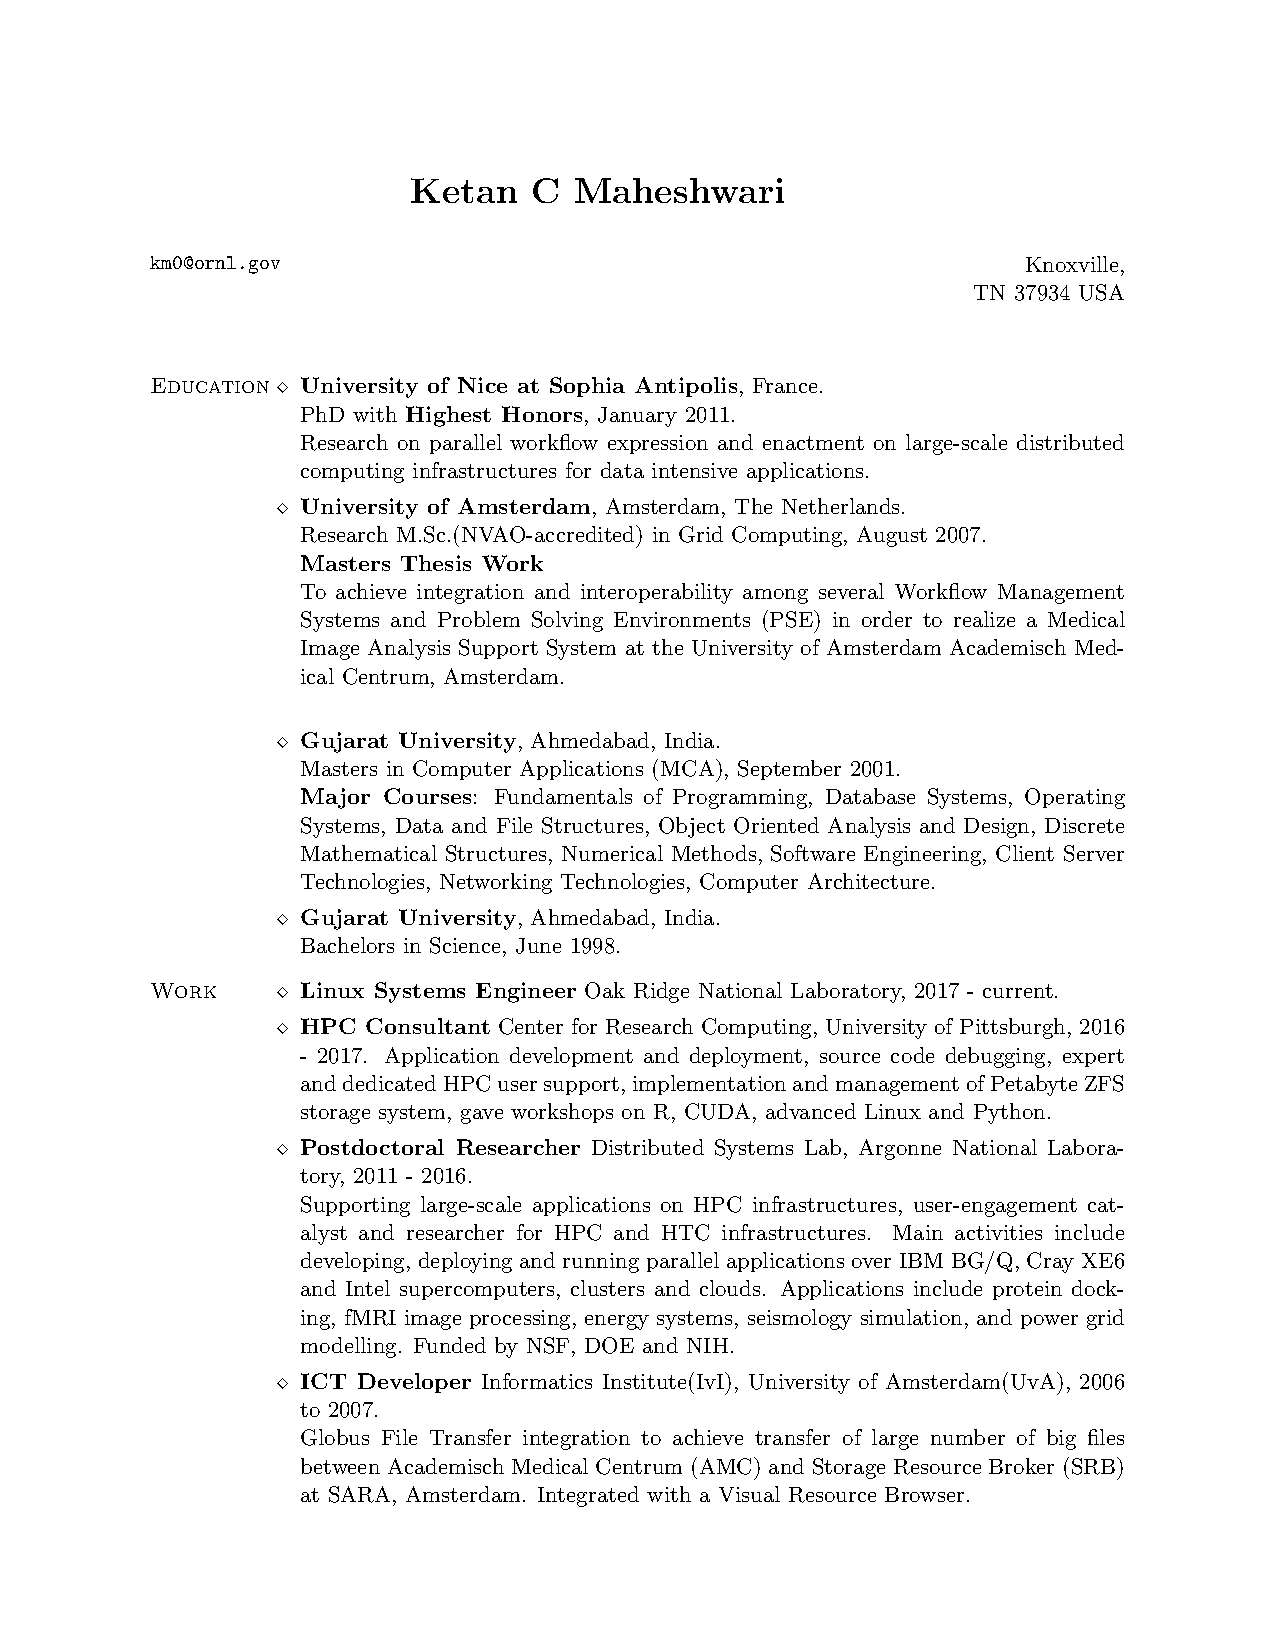
\includepdf[pages=-,pagecommand={}]{ketanbio.pdf}
\includepdf[pages=-,pagecommand={}]{HongResume.pdf}

\end{document}

Audience and Benefits

yum, apt, dnf etc. are ok on VMs and Desktops but not on clusters. Why?

Understanding a Makefile and make commands
VERBOSE and parallel with -j
troubleshoot

autotools autoconf
    troubleshoot

configure; make; make install
    troubleshoot

ccmake, cmake, make && make install
    troubleshoot

Environment variables

Compilers times Libraries times versions

update / upgrade software

The python zoo

userspace rpms
    rare but possible

dangers and pitfalls
system-level libraries
best practices

java ant apache build

binary installations

